%package list
\documentclass{article}
\usepackage[top=3cm, bottom=3cm, outer=3cm, inner=3cm]{geometry}
\usepackage{multicol}
\usepackage{graphicx}
\usepackage{url}
%\usepackage{cite}
\usepackage{hyperref}
\usepackage{array}
%\usepackage{multicol}
\newcolumntype{x}[1]{>{\centering\arraybackslash\hspace{0pt}}p{#1}}
\usepackage{natbib}
\usepackage{pdfpages}
\usepackage{multirow}
\usepackage[normalem]{ulem}
\useunder{\uline}{\ul}{}
\usepackage{svg}
\usepackage{xcolor}
\usepackage{listings}
\lstdefinestyle{ascii-tree}{
    literate={├}{|}1 {─}{--}1 {└}{+}1 
  }
\lstset{basicstyle=\ttfamily,
  showstringspaces=false,
  commentstyle=\color{red},
  keywordstyle=\color{blue}
}
%\usepackage{booktabs}
\usepackage{caption}
\usepackage{subcaption}
\usepackage{float}
\usepackage{array}

\newcolumntype{M}[1]{>{\centering\arraybackslash}m{#1}}
\newcolumntype{N}{@{}m{0pt}@{}}


%%%%%%%%%%%%%%%%%%%%%%%%%%%%%%%%%%%%%%%%%%%%%%%%%%%%%%%%%%%%%%%%%%%%%%%%%%%%
%%%%%%%%%%%%%%%%%%%%%%%%%%%%%%%%%%%%%%%%%%%%%%%%%%%%%%%%%%%%%%%%%%%%%%%%%%%%
\newcommand{\itemEmail}{vmamanian@unsa.edu.pe}
\newcommand{\itemStudent}{Victor Mamani Anahua}
\newcommand{\itemCourse}{Fundamentos de la Programación II}
\newcommand{\itemCourseCode}{20230489}
\newcommand{\itemSemester}{II}
\newcommand{\itemUniversity}{Universidad Nacional de San Agustín de Arequipa}
\newcommand{\itemFaculty}{Facultad de Ingeniería de Producción y Servicios}
\newcommand{\itemDepartment}{Departamento Académico de Ingeniería de Sistemas e Informática}
\newcommand{\itemSchool}{Escuela Profesional de Ingeniería de Sistemas}
\newcommand{\itemAcademic}{2023 - B}
\newcommand{\itemInput}{Del 04 Diciembre 2023}
\newcommand{\itemOutput}{Al 11 Diciembre 2023}
\newcommand{\itemPracticeNumber}{12}
\newcommand{\itemTheme}{Laboratorio 12}
%%%%%%%%%%%%%%%%%%%%%%%%%%%%%%%%%%%%%%%%%%%%%%%%%%%%%%%%%%%%%%%%%%%%%%%%%%%%
%%%%%%%%%%%%%%%%%%%%%%%%%%%%%%%%%%%%%%%%%%%%%%%%%%%%%%%%%%%%%%%%%%%%%%%%%%%%

\usepackage[english,spanish]{babel}
\usepackage[utf8]{inputenc}
\AtBeginDocument{\selectlanguage{spanish}}
\renewcommand{\figurename}{Figura}
\renewcommand{\refname}{Referencias}
\renewcommand{\tablename}{Tabla} %esto no funciona cuando se usa babel
\AtBeginDocument{%
	\renewcommand\tablename{Tabla}
}

\usepackage{fancyhdr}
\pagestyle{fancy}
\fancyhf{}
\setlength{\headheight}{30pt}
\renewcommand{\headrulewidth}{1pt}
\renewcommand{\footrulewidth}{1pt}
\fancyhead[L]{\raisebox{-0.2\height}{
\includegraphics[width=3cm]{img/logo_episunsa.png}}}
\fancyhead[C]{\fontsize{7}{7}\selectfont	\itemUniversity \\ \itemFaculty \\ \itemDepartment \\ \itemSchool \\ \textbf{\itemCourse}}
\fancyhead[R]{\raisebox{-0.2\height}{
\includegraphics[width=1.2cm]{img/logo_abet}}}
\fancyfoot[L]{Estudiante Victor Mamani A.}
\fancyfoot[C]{\itemCourse}
\fancyfoot[R]{Página \thepage}

% para el codigo fuente
\usepackage{listings}
\usepackage{color, colortbl}
\definecolor{dkgreen}{rgb}{0,0.6,0}
\definecolor{gray}{rgb}{0.5,0.5,0.5}
\definecolor{mauve}{rgb}{0.58,0,0.82}
\definecolor{codebackground}{rgb}{0.95, 0.95, 0.92}
\definecolor{tablebackground}{rgb}{0.8, 0, 0}

\lstdefinestyle{java}{frame=tb,
	language=Java,
	showstringspaces=false,
	columns=flexible,
	basicstyle={\footnotesize\ttfamily\color[RGB]{255,255,255}},
	numberstyle=\color{mygray},
	numbers=left, 
	keywordstyle=\color{myblue},
	morekeywords={String, System},
	commentstyle=\color{mygray},
	stringstyle=\color{mygreen},
	breaklines=true,
	breakatwhitespace=true,
	tabsize=2,
	backgroundcolor= \color{codebackgroundCode},
	showspaces=false,
	showtabs=false,
	showlines=false,
}

\lstset{frame=tb,
	language=bash,
	aboveskip=3mm,
	belowskip=3mm,
	showstringspaces=false,
	columns=flexible,
	basicstyle={\small\ttfamily},
	numbers=none,
	numberstyle=\tiny\color{gray},
	keywordstyle=\color{blue},
	commentstyle=\color{dkgreen},
	stringstyle=\color{mauve},
	breaklines=true,
	breakatwhitespace=true,
	tabsize=3,
	backgroundcolor= \color{codebackground},
}

\begin{document}
	
	\vspace*{10px}
	
	\begin{center}	
		\fontsize{17}{17} \textbf{ Informe de Laboratorio \itemPracticeNumber}
	\end{center}
	\centerline{\textbf{\Large Tema: \itemTheme}}
	%\vspace*{0.5cm}	

	\begin{flushright}
		\begin{tabular}{|M{2.5cm}|N|}
			\hline 
			\rowcolor{tablebackground}
			\color{white} \textbf{Nota}  \\
			\hline 
			     \\[30pt]
			\hline 			
		\end{tabular}
	\end{flushright}	

	\begin{table}[H]
		\begin{tabular}{|x{4.7cm}|x{4.8cm}|x{4.8cm}|}
			\hline 
			\rowcolor{tablebackground}
			\color{white} \textbf{Estudiante} & \color{white}\textbf{Escuela}  & \color{white}\textbf{Asignatura}   \\
			\hline 
			{\itemStudent \par \itemEmail} & \itemSchool & {\itemCourse \par Semestre: \itemSemester \par Código: \itemCourseCode}     \\
			\hline 			
		\end{tabular}
	\end{table}		
	
	\begin{table}[H]
		\begin{tabular}{|x{4.7cm}|x{4.8cm}|x{4.8cm}|}
			\hline 
			\rowcolor{tablebackground}
			\color{white}\textbf{Laboratorio} & \color{white}\textbf{Tema}  & \color{white}\textbf{Duración}   \\
			\hline 
			\itemPracticeNumber & \itemTheme & 04 horas   \\
			\hline 
		\end{tabular}
	\end{table}
	
	\begin{table}[H]
		\begin{tabular}{|x{4.7cm}|x{4.8cm}|x{4.8cm}|}
			\hline 
			\rowcolor{tablebackground}
			\color{white}\textbf{Semestre académico} & \color{white}\textbf{Fecha de inicio}  & \color{white}\textbf{Fecha de entrega}   \\
			\hline 
			\itemAcademic & \itemInput &  \itemOutput  \\
			\hline 
		\end{tabular}
	\end{table}
	
	\section{Tarea}
	\begin{itemize}		
        \item Cree un Proyecto llamado Laboratorio12.
        \item Puede reutilizar todo el código del laboratorio 11, pero ahora el objetivo es gestionar los ejércitos autogenerados.
        \item Al ejecutar el videojuego, el programa deberá dar las opciones:
        \item 1. Juego rápido (tal cual como en el laboratorio 11) Al acabar el juego mostrar las opciones de volver a jugar y de volver al	menú principal. También se deberá tener la posibilidad de cancelar el juego actual en cualquier momento, permitiendo escoger entre empezar un juego totalmente nuevo o salir al menú principal.
        \item 2. Juego personalizado: permite gestionar ejércitos. Primero se generan los 2 ejércitos con sus respectivos soldados y se muestran sus datos	Luego se tendrá que escoger cuál de los 2 ejércitos se va a gestionar, después se mostrarán las siguientes opciones:
		\item -1- Crear Soldado: permitirá crear un nuevo soldado personalizado y añadir al final del ejército (recordar que límite es de 10 soldados por ejército)s.
		\item -2- Eliminar Soldado (no debe permitir un ejército vacío)
		\item -3- Clonar Soldado (crea una copia exacta del soldado) y se añade al final del ejército (recordar que límite es de 10 soldados por ejército)
		\item -4- Modificar Soldado (con submenú para cambiar alguno de los	atributos nivelAtaque, nivelDefensa, vidaActual)
		\item -5- Comparar Soldados (verifica si atributos: nombre, nivelAtaque, nivelDefensa, vidaActual y vive son iguales)
		\item -6- Intercambiar Soldados (intercambia 2 soldados en sus posiciones en la estructura de datos del ejército)
		\item -7- Ver soldado (Búsqueda por nombre)
		\item -8- Ver ejército
		\item -9- Sumar niveles (usando Method-Call Chaining), calcular las sumatorias de nivelVida, nivelAtaque, nivelDefensa, velocidad de todos los soldados de un ejército 1. Por ejemplo, si ejército tendría 3 soldados:
		2. s=s1.sumar(s2).sumar(s3);
		3. s es un objeto Soldado nuevo que contendría las
		sumatorias de los 4 atributos indicados de los 3 soldados.
		Ningún soldado cambia sus valores
		\item -10- Jugar (se empezará el juego con los cambios realizados) y con las mismas opciones de la opción 1.
		\item -11- Volver (muestra el menú principal) Después de escoger alguna de las opciones -1- a -9- se podrá volver a elegir uno de los ejércitos y se mostrarán las opciones -1- a -11-
		\end{itemize}

	\section{Equipos, materiales y temas utilizados}
	\begin{itemize}
		\item Sistema Operativo Ubuntu GNU Linux 23 lunar 64 bits Kernell 6.2.v
		\item Visual Studio Code.
		\item VIM 9.0.
		\item OpenJDK 64-Bits 19.0.7.
		\item Git 2.39.2.
		\item Cuenta en GitHub con el correo institucional.
		\item Programación Orientada a Objetos.
		\item Actividades del Laboratorio 12.	
	\end{itemize}
	
	\section{URL de Repositorio Github}
	\begin{itemize}
		\item URL del Repositorio GitHub para clonar o recuperar.
		\item \url{https://github.com/VictorMA18/fp2-23b.git}
		\item URL para el laboratorio 12 en el Repositorio GitHub.
		\item \url{https://github.com/VictorMA18/fp2-23b/tree/main/Fase02/Lab12}
	\end{itemize}
	
	\section{Actividades del Laboratorio 12}

	\subsection{Ejercicio Soldado}
	\begin{itemize}	
		\item En el primer commit agregando la clase soldado que esta siendo reutilizada para podef reslizar el siguiente ejercicio.
		\item El codigo y el commit seria el siguiente:
	\end{itemize}	
	\begin{lstlisting}[language=bash,caption={Commit}][H]
		$ git commit -m "Agregando la clase soldado para podef reslizar el siguiente ejercicio "
	\end{lstlisting}	
	\begin{lstlisting}[language=java,caption={Las lineas de codigos del metodo creado:}][H]
		// Laboratorio Nro 12 - Ejercicio Soldado
		// Autor: Mamani Anahua Victor Narciso
		// Colaboro:
		// Tiempo:
		import java.util.*;
		public class Soldado { //CREAMOS LA CLASE SOLDODADO PARA PODER USAR UN ARREGLO BIDIMENSIONAL DONDE NECESITAMOS LA VIDA , EL NOMBRE DEL SOLDADO Y TAMBIEN SU POSICION COMO LA FILA Y LA COLUMNA   
		
			private String name;
			private int lifeactual;
			private int row;
			private String column;
			private int attacklevel;
			private int defenselevel;
			private int lifelevel;
			private int speed;
			private String attitude;
			private boolean lives;
		
			Random rdm = new Random();
		
			//Anadiendo metodo que nos permita que un arreglo tenga datos nulos si este esta vacio
			public Soldado(){
				this.name = "";
				this.row = 0;
				this.column  = "";
				this.attacklevel = 0;
				this.defenselevel = 0;
				this.lifelevel = 0;
				this.lifeactual = 0;
				this.speed = 0;
				this.attitude = "";
				this.lives = false;
			}
		
			//Constructor
			public Soldado(String name, int health, int row, String column){
				this.name = name;
				this.lifeactual = health;
				this.lifelevel = health;
				this.lifeactual = health;
				this.row = row;
				this.column = column;
				this.lives = true;
				
				//YA QUE ESTOS DATOS SERIAN ALEATORIOS YA QUE SE ESTARIA CREANDO EL SOLDADO TENDRIAMOS DATOS QUE SERIAN COMO ATTACKLEVEL DEFENSELEVEL EL CUAL TENDRIAN QUE SER ALEATORIOS    
				this.attacklevel = rdm.nextInt(5) + 1;
				this.defenselevel = rdm.nextInt(5) + 1;
		
			}
			
			//Constructor para los diferentes niveles como de vidad defensa ataque velocidad
			public Soldado(String name , int attacklevel, int defenselevel, int lifelevel, int speed, boolean lives, int row, String column) {
				this.name = name;
				this.attacklevel = attacklevel;
				this.defenselevel = defenselevel;
				this.lifelevel = lifelevel;
				this.speed = speed;
				this.lives = lives;
				this.row = row;
				this.column = column;
			}
		
			//Metodos necesarios como avanzar defender huir al seratacado al retroceder
			public void advance(){
				this.speed = getSpeed() + 1;
				System.out.println("El soldado " + this.name + "avanzo");
			}
			public void defense(){
				this.speed = 0;
				this.attitude = "DEFENSIVA";
				System.out.println("El soldado " + this.name + "esta defendiendo");
			}
			public void flee(){
				this.speed = getSpeed() + 2;
				this.attitude = "HUYE";
				System.out.println("El soldado " + this.name + "esta huyendo");
			}
			public void back(){
				System.out.println("El soldado " + this.name + "esta retrocediendo");
				if(this.speed == 0){
					this.speed = rdm.nextInt(5) - 5;
				}else{
					if(this.speed > 0){
						this.speed = 0;
						this.attitude = "DEFENSIVA";
					}
				}
			}
			public void attack(Soldado soldier){
				if(this.getLifeActual() > soldier.getLifeActual()){
					int life = this.getLifeActual() - soldier.getLifeActual();
					this.setLifeActual(life);
					this.setLifeLevel(life);
					soldier.lives = false;
					soldier.morir();
					System.out.println(this.name + " asesino al soldado " + soldier.name);
				}else if(soldier.getLifeActual() > this.getLifeActual()){
					int life = soldier.getLifeActual() - this.getLifeActual();
					this.lives = false;
					this.morir();
					soldier.setLifeActual(life);
					soldier.setLifeLevel(life);
					System.out.println(soldier.name + " asesino al soldado " + this.name);
				}else{
					this.lives = false;
					this.morir();   
					soldier.lives = false;
					soldier.morir();
					System.out.println("los 2 soldados se asesinaron");
				}
			}
			public void morir(){
				this.lives = false;
				this.attitude = "SOLDADO MUERTO";
			}
		
			// Metodos mutadores
			public void setName(String n){
				name = n;
			}
			public void setLifeActual(int p){
				lifeactual = p;
			}
			public void setRow(int b){
				row = b;
			}
			public void setColumn(String c){
				column = c; 
			}
			public void setAttackLevel(int attacklevel) {
				this.attacklevel = attacklevel;
			}
			public void setDefenseLevel(int defenselevel) {
				this.defenselevel = defenselevel;
			}
			public void setLifeLevel(int lifelevel){
				this.lifelevel = lifelevel;
			}
			public void setSpeed(int speed) {
				this.speed = speed;
			}
			public void setAttitude(String attitude) {
				this.attitude = attitude;
			}
			public void setLives(boolean lives) {
				this.lives = lives;
			}
		
			// Metodos accesores
			public String getName(){
				return name;
			}
			public int getLifeActual(){
				return lifeactual;
			}
			public int getRow(){
				return row;
			}
			public String getColumn(){
				return column;
			}
			public int getAttackLevel() {
				return attacklevel;
			}
			public int getDefenseLevel() {
				return defenselevel;
			}
			public int getLifeLevel(){
				return lifelevel;
			}
			public int getSpeed() {
				return speed;
			}
			public String getAttitude() {
				return attitude;
			}
			public boolean getLives() {
				return lives;
			}
		
			// Completar con otros metodos necesarios
			public String toString(){ //CREAMOS ESTE METODO PARA IMPRIMIR LOS DATOS DEl OBJETO
				String join = "\nNombre: " + getName() + "\nVida: " + getLifeActual() + "\nFila: " + getRow() + "\nColumna: " + getColumn() + "\nNivel de ataque: " + getAttackLevel() + "\nNivel de Defensa: " + getDefenseLevel() + "\nNivel de vida: " + getLifeLevel() + "\nVelocidad: " + getSpeed() + "\nActitud: " + getAttitude() + "\nEstado: " + getLives(); //Agregamos un espaciador para poder separar
				return join;
			}
		}		

	\end{lstlisting}
	\subsection{Ejercicio Videojuego2}
	\begin{itemize}	
		\item En el segundo commit ponemos las cosas necesarias que se requirio para el lab12 que era que tenemos que reutilizar el lab11 y en el lab11 se dice que las batallas entre 2 soldados sse define por su nivel de probabilidad asi imprimendolo para mostrar el resultado de esa batalla
		\item El codigo y el commit seria el siguiente:
	\end{itemize}	
	\begin{lstlisting}[language=bash,caption={Commit}][H]
		$ git commit -m " Poniendo las funciones del laboratorio 11 las cuales se pedian para hacer este lab por ejemplo las batallas entre 2 soldados y el resultado de estas mediante porcentajes de probabilidad"
	\end{lstlisting}	
	\begin{lstlisting}[language=java,caption={Las lineas de codigos del metodo creado:}][H]
		if(health2 > health1){
            double sumhealth = (health2 + health1) * 1.0;
            System.out.println("\n \t Resultado de la Batalla");
            System.out.println("El soldado del bando X es el ganador ya que su probabilidad de ganar la batalla es --> " +  String.format( "%.1f" , ((health2/sumhealth) * 1000 ) / 10)  + "% y la probabilidad del soldado del bando Y es ---> " + String.format( "%.1f" , ((health1/sumhealth) * 1000) / 10) + "%" );
		}
		else if(health1 > health2){
			double sumhealth = (health2 + health1) * 1.0; 
			System.out.println("\n \t Resultado de la Batalla");
			System.out.println("El soldado del bando Y es el ganador ya que su probabilidad de ganar la batalla es --> " +  String.format( "%.1f" , ((health1/sumhealth) * 1000 ) / 10)  + "% y la probabilidad del soldado del bando X es ---> " + String.format( "%.1f" , ((health2/sumhealth) * 1000) / 10) + "%" );
		}
	\end{lstlisting}
	\begin{figure}[H]
		\centering
		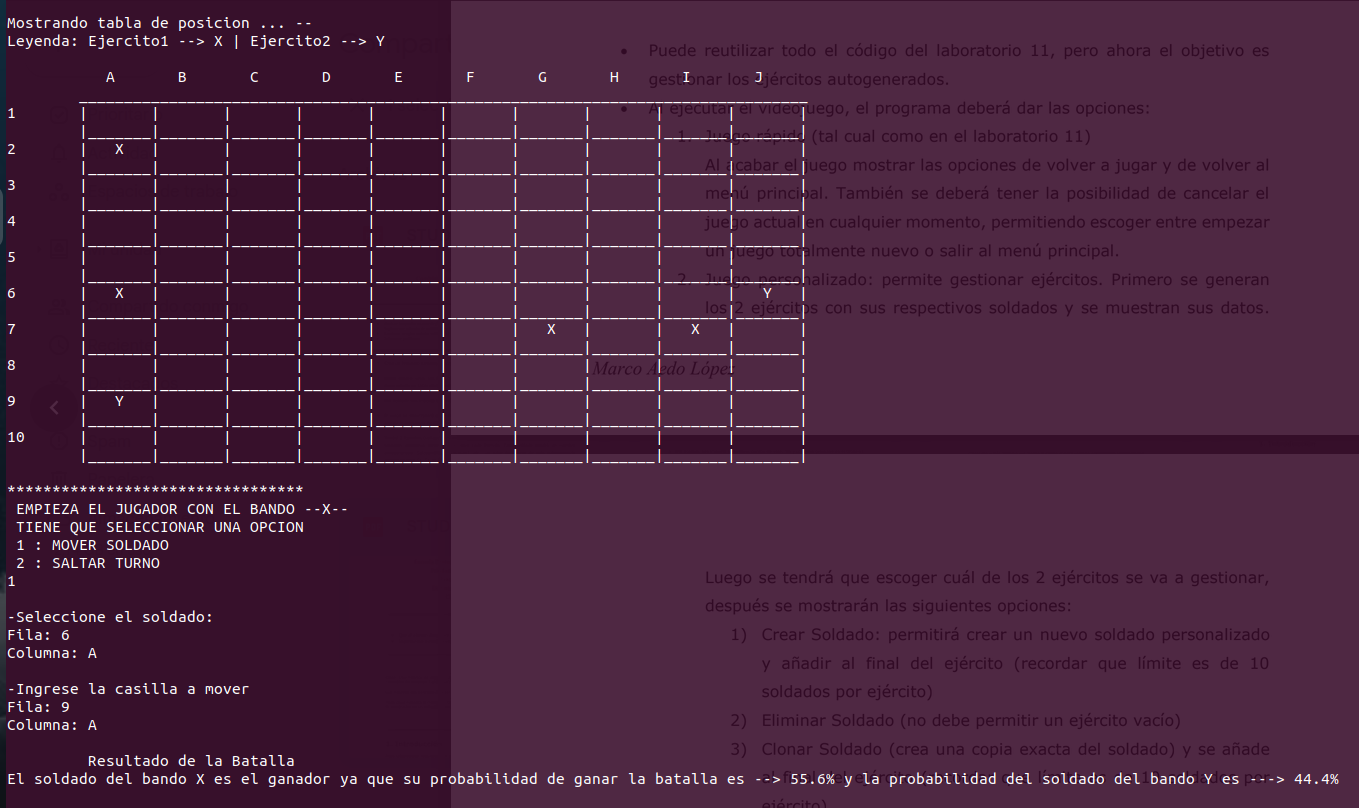
\includegraphics[width=1.0\textwidth,keepaspectratio]{img/Commit2.png}
		%\includesvg{img/automata.svg}
		%\label{img:mot2}
		%\caption{Product backlog.}
	\end{figure}
	\begin{figure}[H]
		\centering
		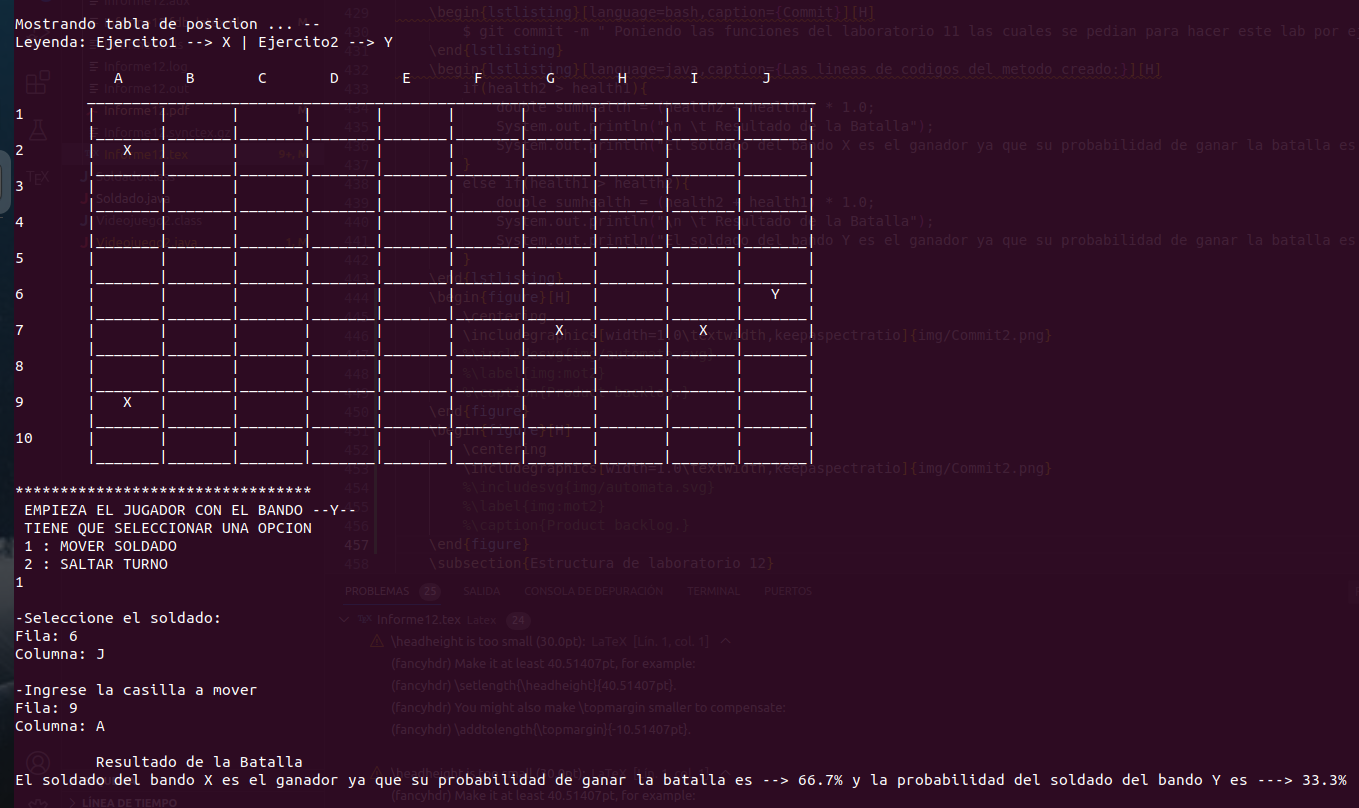
\includegraphics[width=1.0\textwidth,keepaspectratio]{img/Commit2.1.png}
		%\includesvg{img/automata.svg}
		%\label{img:mot2}
		%\caption{Product backlog.}
	\end{figure}
	\subsection{Ejercicio Videojuego2}
	\begin{itemize}	
		\item En el tercer commit agregamos opciones para tener un juego rapido o personalizado para esto creamos una funcion la cual nos ayudara  
		\item El codigo , el commit y ejecución seria el siguiente:
	\end{itemize}	
	\begin{lstlisting}[language=bash,caption={Commit}][H]
		$ git commit -m "El juego ya tendria opciones de juego si fuera un juego rapido falta el personalizado se agregan opciones para ver cual de estas se quiere jugar"
	\end{lstlisting}	
	\begin{lstlisting}[language=java,caption={Las lineas de codigos del metodo creado:}][H]
		public static void optionsbattle(ArrayList<ArrayList<Soldado>> army1 , ArrayList<ArrayList<Soldado>> army2){
			Scanner sc = new Scanner(System.in);
			System.out.println("-------------------------------------------");
			System.out.println("--          OPCIONES DE BATALLA          --"); 
			System.out.println("-------------------------------------------");
			System.out.println(" SELECCIONE UN NUMERO PARA PODER EMPEZAR O TERMINAR");
			System.out.println(" 1 : JUEGO RAPIDO");
			System.out.println(" 2 : JUEGO PERSONALIZADO");
			int optbattle = sc.nextInt();
			if(optbattle == 1){
				battle(army1, army2);
			}else{
	
			}
		}
	\end{lstlisting}
	\begin{figure}[H]
		\centering
		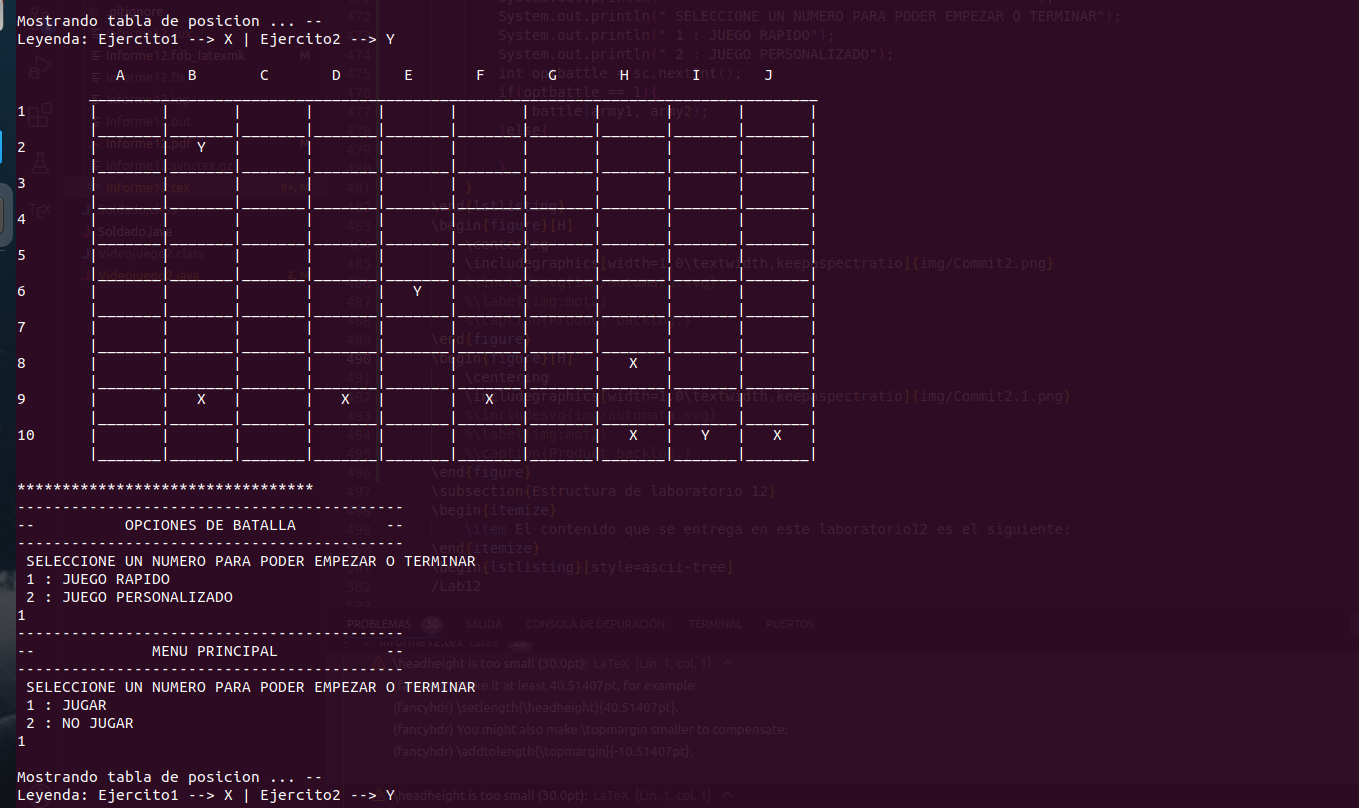
\includegraphics[width=1.0\textwidth,keepaspectratio]{img/Commit3.png}
		%\includesvg{img/automata.svg}
		%\label{img:mot2}
		%\caption{Product backlog.}
	\end{figure}
	\subsection{Ejercicio Videojuego2}
	\begin{itemize}	
		\item En el cuarto commit agregamos opciones para el jeugo personalizado estas serian como la primera opcion la cual nos ayuda a crear un soldado para el ejercito para esto hacemos un do while el cual nos ayudara con las opciones que quiera escoger el jugador y en esta opcion de crear el jugador ponemos la condicion de que no sobrepase el maximo de soldados el cual seria 10 soldados para este soldado creado le ponemos un nombre una vida y su ubicacion en el mapa.  
		\item El codigo y el commit seria el siguiente:
	\end{itemize}	
	\begin{lstlisting}[language=bash,caption={Commit}][H]
		$ git commit -m "Creando la primera opcion del Juego personalizado"
	\end{lstlisting}	
	\begin{lstlisting}[language=java,caption={Las lineas de codigos del metodo creado:}][H]
		public static void battlePersonalized(ArrayList<ArrayList<Soldado>> army1 , ArrayList<ArrayList<Soldado>> army2){
			Scanner sc = new Scanner(System.in);
			System.out.println("Gestionar Ejercito \n[1] Ejercito 1\n[2] Ejercito 2");
			int optarmy = sc.nextInt();
			do {
				System.out.println("Escoja una de estas opciones para el ejercito 1");
				System.out.println("[1] Crear Soldado"+
									"\n[2] Eliminar Soldado" + 
									"\n[3] Clonar Soldado"+
									"\n[4] Modificar Soldado"+
									"\n[5] Comparar Soldados"+
									"\n[6] Intercambiar Soldados"+
									"\n[7] Ver soldado"+
									"\n[8] Ver ejercito"+
									"\n[9] Sumar Niveles"+
									"\n[10] Jugar" +
									"\n[11] Volver");
				int optPersonalized = sc.nextInt();
				switch (optPersonalized) {
					case 1:
						int numbersoldiers = 0;
						for(int i = 0; i < 10; i++){  //ITERACION CREADA PARA PODER SABER QUE SI ESTE BANDO DEL EJERCITO TIENE SOLDADOS PARA PODER JUGAR SI TIENE 10 ESTA OPCION ESTA CANCELADA
							for(int j = 0; j < 10; j++){
								if(army1.get(i).get(j) != null){
									numbersoldiers++;
								}
							}
						}
						if(numbersoldiers == 10){
							System.out.println("USTED NO PUEDE CREAR MAS SOLDADOS EL MAXIMO ES 10 SOLDADOS POR EJERCITO");
						}else{
							String name = sc.next();
							int health = sc.nextInt();
							int row = sc.nextInt() - 1;
							String column = sc.next();
							Soldado soldier =  new Soldado(name, health, numbersoldiers, column);
							army1.get(row).set((int)column.charAt(0) - 65, soldier);
						}
						viewBoard(army1, army2);
						break;
					default:
						break;
				}
				
			} while (optarmy == 1);
		}
	\end{lstlisting}
	\begin{figure}[H]
		\centering
		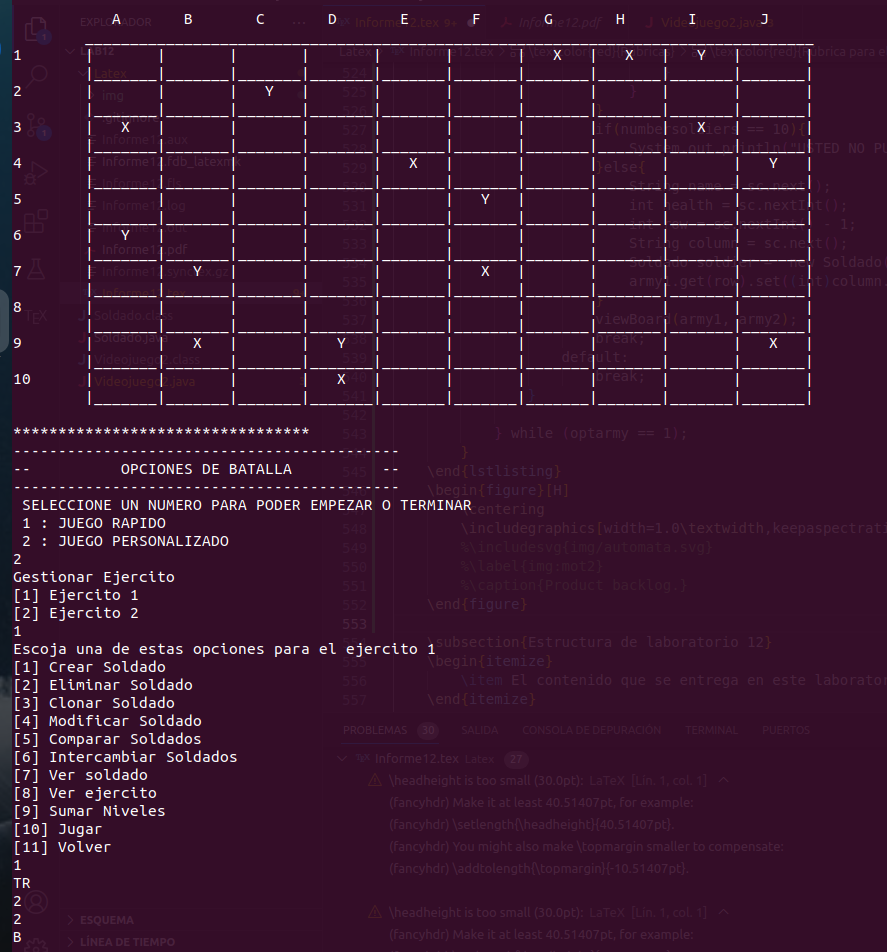
\includegraphics[width=1.0\textwidth,keepaspectratio]{img/Commit4.0.png}
		%\includesvg{img/automata.svg}
		%\label{img:mot2}
		%\caption{Product backlog.}
	\end{figure}
	\begin{figure}[H]
		\centering
		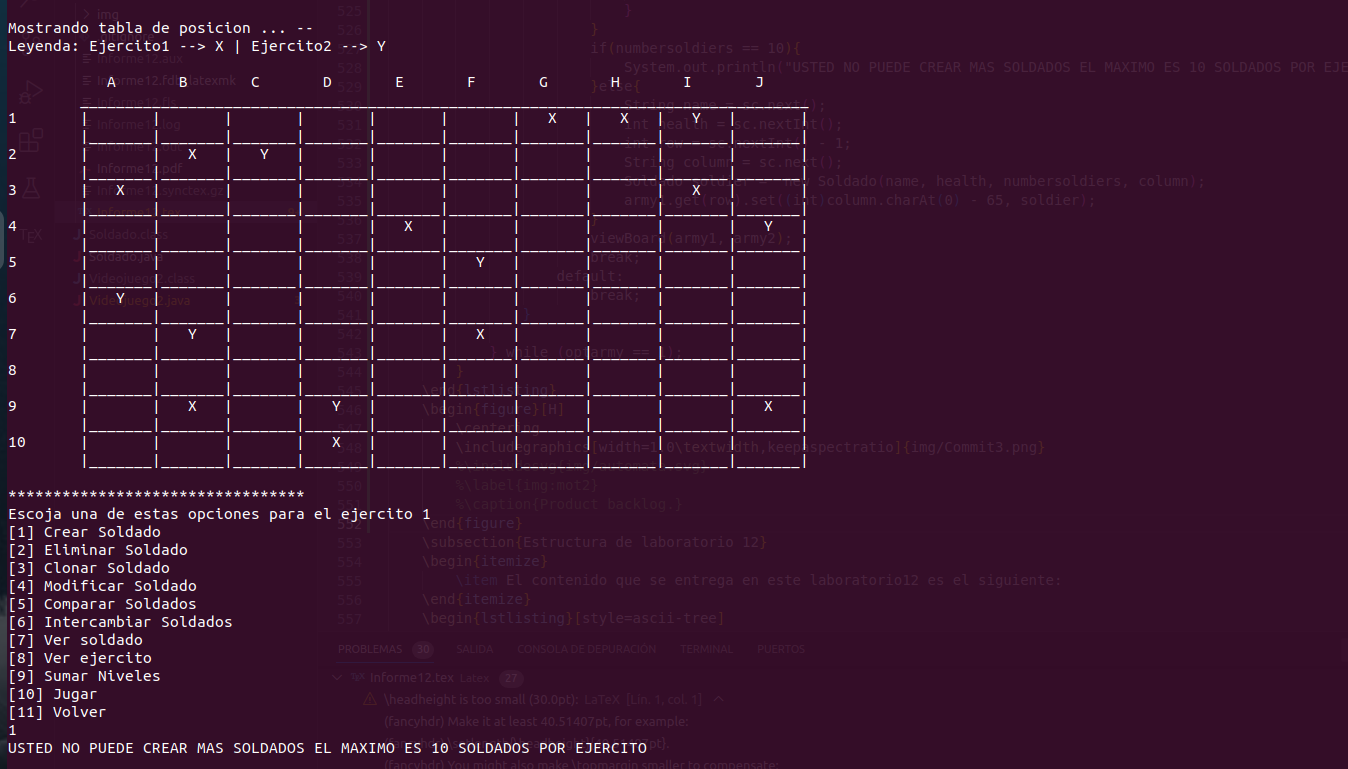
\includegraphics[width=1.0\textwidth,keepaspectratio]{img/Commit4.1.png}
		%\includesvg{img/automata.svg}
		%\label{img:mot2}
		%\caption{Product backlog.}
	\end{figure}
	\subsection{Ejercicio Videojuego2}
	\begin{itemize}	
		\item En el quinto commit agregamos la opcion numero 2 la cual nos va poder permitir eliminar a un soldado del ejercito para esto hacemos una comprobacion y elminamos al soldado requerido mediante su ubicacion con eso vaciariamos su posicion y tambien con esta opcion no permitimos que este ejercito se autoelimine por no tener soldados anquesea vamos a dejar 1 soldado en sus filas.
		\item El codigo y el commit seria el siguiente:
	\end{itemize}	
	\begin{lstlisting}[language=bash,caption={Commit}][H]
		$ git commit -m "Dando la opcion numero 2 al juego persolnalizado la cual es eliminar a un soldado del ejercito pero sin que este ejercito se vacie para esto hacemos una condicion la cual nos va poder decir que esta anquesea va a tener 1 soldado en sus filas"
	\end{lstlisting}	
	\begin{lstlisting}[language=java,caption={Las lineas de codigos del metodo creado:}][H]
		case 2:
			numbersoldiers = 0;
			for(int i = 0; i < 10; i++){  //ITERACION CREADA PARA PODER SABER QUE SI ESTE BANDO DEL EJERCITO TIENE SOLDADOS PARA PODER JUGAR SI TIENE 10 ESTA OPCION ESTA CANCELADA
				for(int j = 0; j < 10; j++){
					if(army1.get(i).get(j) != null){
						numbersoldiers++;
					}
				}
			}
			if(numbersoldiers == 1){
				System.out.println("*********************************");
				System.out.println("USTED NO PUEDE ELIMINAR MAS SOLDADOS YA QUE ELIMINARIA A SU EJERCITO");    
			}else{
				System.out.println("*********************************");
				System.out.println("Escriba la fila donde esta el soldado el cual eliminara:");
				int row = sc.nextInt() - 1;
				System.out.println("Escriba la columna donde esta el soldado el cual eliminara:");
				String column = sc.next();
				army1.get(row).set((int)column.charAt(0) - 65, null);
			}
			viewBoard(army1, army2);
			break;
	\end{lstlisting}
	\begin{figure}[H]
		\centering
		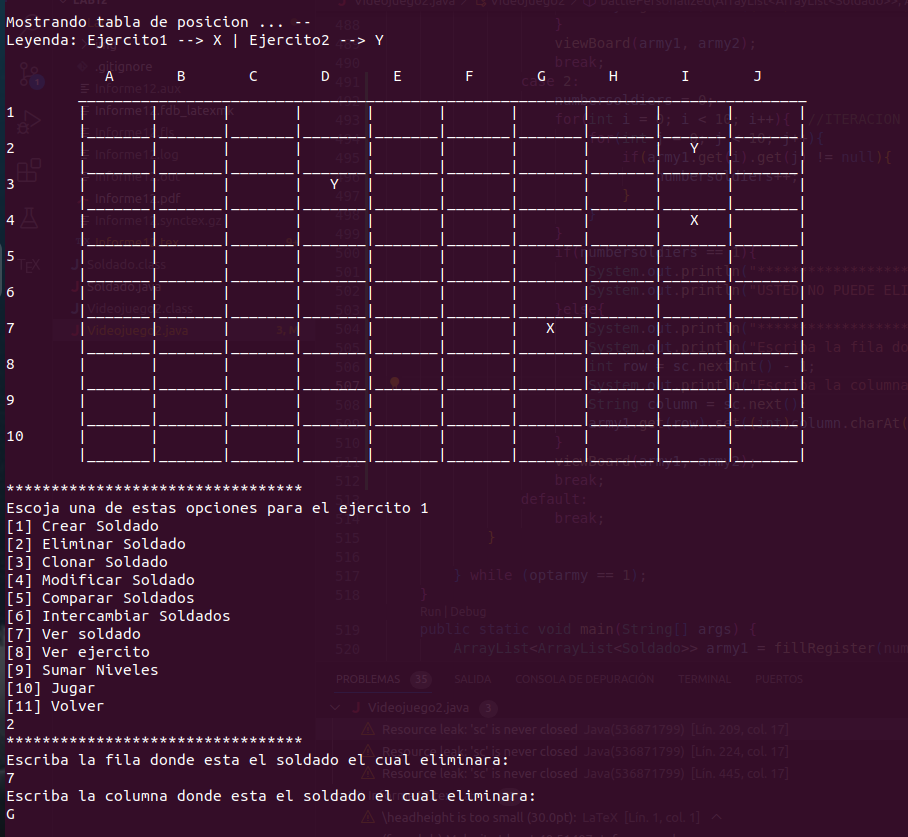
\includegraphics[width=1.0\textwidth,keepaspectratio]{img/Commit5.png}
		%\includesvg{img/automata.svg}
		%\label{img:mot2}
		%\caption{Product backlog.}
	\end{figure}
	\begin{figure}[H]
		\centering
		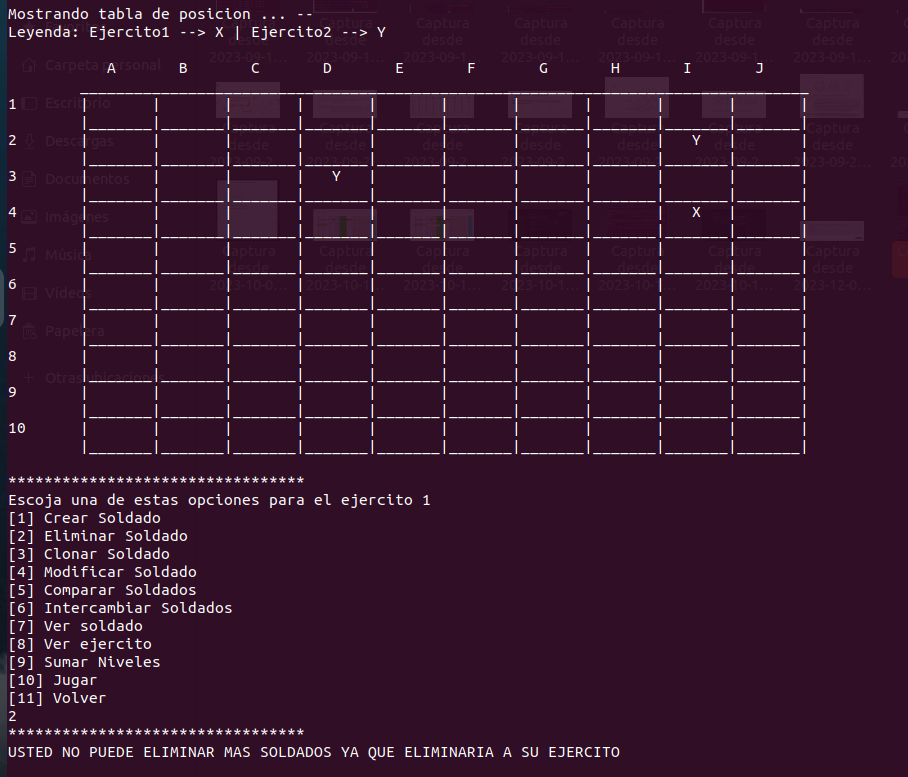
\includegraphics[width=1.0\textwidth,keepaspectratio]{img/Commit5.1.png}
		%\includesvg{img/automata.svg}
		%\label{img:mot2}
		%\caption{Product backlog.}
	\end{figure}
	\subsection{Ejercicio Videojuego2}
	\begin{itemize}	
		\item En el sexto commit agregamos la opcion numero 3 la cual nos va poder permitir clonar a un soldado del ejercito para esto hacemos una comprobacion y clonamos al soldado requerido mediante su ubicacion con eso lo ponemos en su posicion donde queremos y tambien con esta opcion no permitimos que este ejercito se llene lo cual seria mas de 10 soldados en un ejercito.
		\item El codigo , el commit y ejecucion seria el siguiente:
	\end{itemize}	
	\begin{lstlisting}[language=bash,caption={Commit}][H]
		$ git commit -m "Agregando la opcion 3 al menu de juego personalizado el cual vamos a tener que comprobar que no sobrepase el numero de soldados que es 10 para poder clonar y ver en el tablero para esto hacemos condiciones y buscamos posiciones de los soldados"
	\end{lstlisting}	
	\begin{lstlisting}[language=java,caption={Las lineas de codigos del metodo creado:}][H]
		case 3:
		numbersoldiers = 0;
		for(int i = 0; i < 10; i++){  //ITERACION CREADA PARA PODER SABER QUE SI ESTE BANDO DEL EJERCITO TIENE SOLDADOS PARA PODER JUGAR SI TIENE 10 ESTA OPCION ESTA CANCELADA
			for(int j = 0; j < 10; j++){
				if(army1.get(i).get(j) != null){
					numbersoldiers++;
				}
			}
		}
		if(numbersoldiers == 10){
			System.out.println("*********************************");
			System.out.println("USTED NO PUEDE CLONAR MAS SOLDADOS EL MAXIMO ES 10 SOLDADOS POR EJERCITO");
		}else{
			System.out.println("Escriba la fila donde esta el soldado que quiere clonar:");
			int row = sc.nextInt() - 1;
			System.out.println("Escriba la columna donde esta el soldado que quiere clonar:");
			String column = sc.next();
			Soldado soldado = army1.get(row).get((char)column.charAt(0) - 65);
			System.out.println("Escriba la fila donde va a estar el soldado que quiere clonar:");
			int rowafter = sc.nextInt() - 1;
			System.out.println("Escriba la columna donde va a estar el soldado que quiere clonar:");
			String columnafter = sc.next();
			army1.get(rowafter).set((char)columnafter.charAt(0) - 65, soldado);
		}
		viewBoard(army1, army2);
	\end{lstlisting}
	\begin{figure}[H]
		\centering
		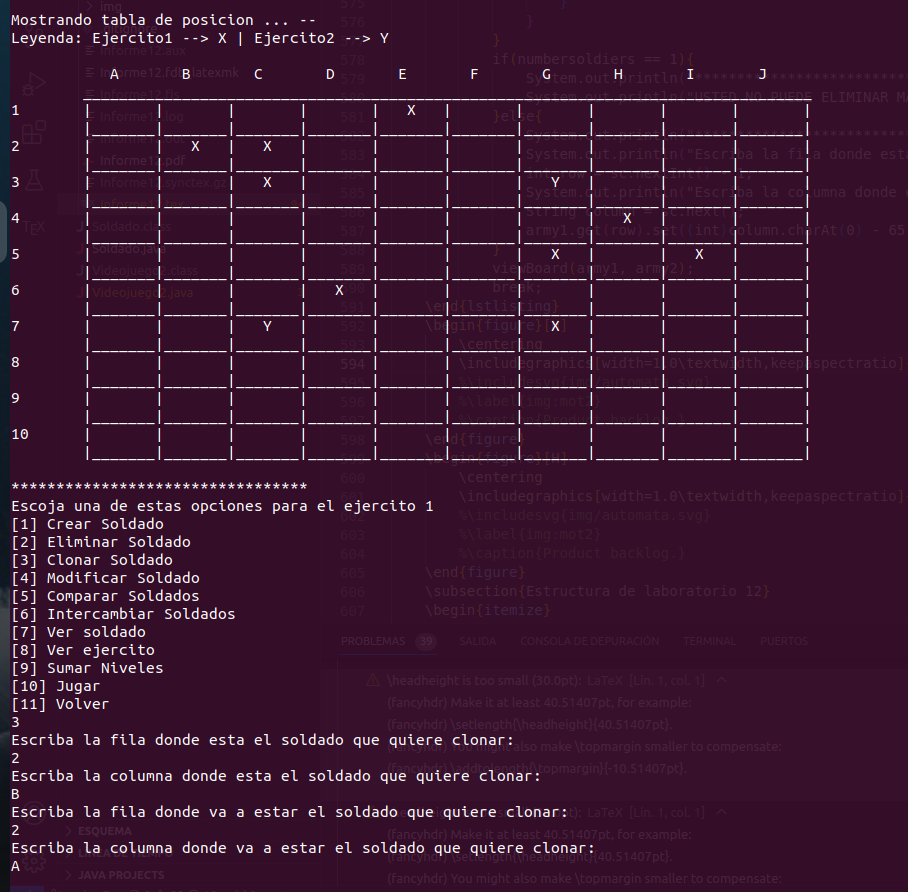
\includegraphics[width=1.0\textwidth,keepaspectratio]{img/Commit6.png}
		%\includesvg{img/automata.svg}
		%\label{img:mot2}
		%\caption{Product backlog.}
	\end{figure}
	\begin{figure}[H]
		\centering
		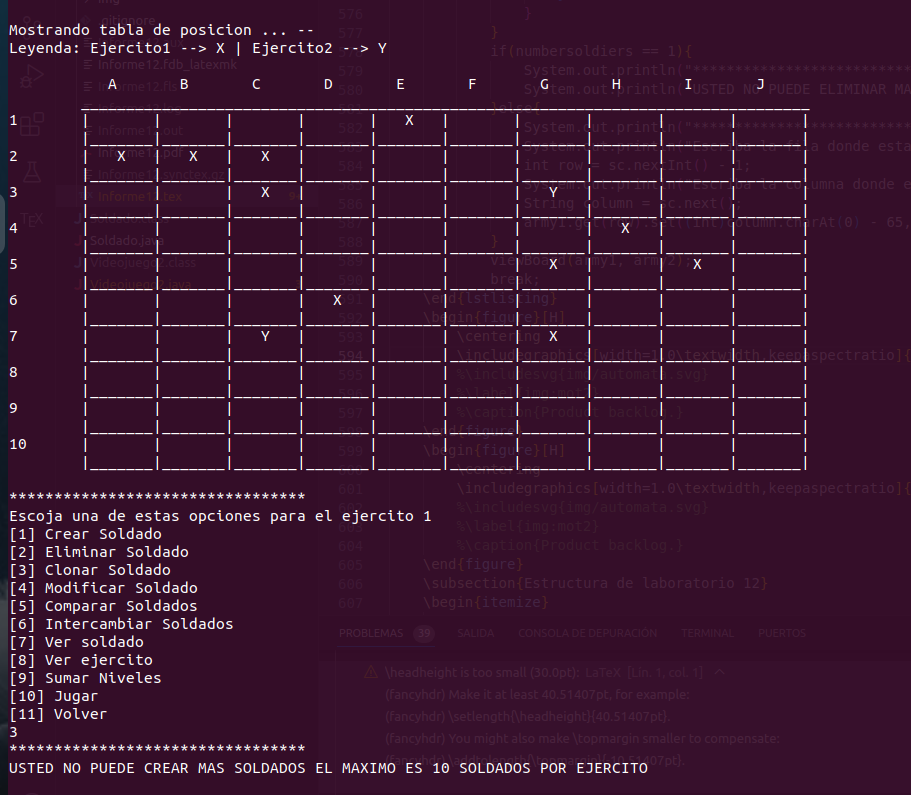
\includegraphics[width=1.0\textwidth,keepaspectratio]{img/Commit6.1.png}
		%\includesvg{img/automata.svg}
		%\label{img:mot2}
		%\caption{Product backlog.}
	\end{figure}
	\subsection{Ejercicio Videojuego2}
	\begin{itemize}	
		\item En el septimo commit agregamos la opcion 4 del menu el cual nos permite cambiar o modificar los atributos del soldado para esto aplicamos de un switch case y tambien imprimimos al soldado para ver sus cambios
		\item El codigo , el commit y ejecucion seria el siguiente:
	\end{itemize}	
	\begin{lstlisting}[language=bash,caption={Commit}][H]
		$ git commit -m "Agregamos la opcion numero 4 para este menu el cual nos permite modificar atributos del soldado el cual escogimos"
	\end{lstlisting}	
	\begin{lstlisting}[language=java,caption={Las lineas de codigos del metodo creado:}][H]
		public static void changeSoldier(ArrayList<ArrayList<Soldado>> army){
			System.out.println("*********************************");
			Scanner sc = new Scanner(System.in);
			System.out.println("Escriba la fila donde esta el soldado el cual modificara:");
			int row = sc.nextInt() - 1;
			System.out.println("Escriba la columna donde esta el soldado el cual modificara:");
			String column = sc.next();
			System.out.println("*********************************");
			System.out.println("QUE DESEA MODIFICAR");
			System.out.println("[1] Nivel de ataque"+
								"\n[2] Nivel de defensa" + 
								"\n[3] Nivel de vida Actual");
			int optchangesoldier = sc.nextInt();
			System.out.println("*********************************");
			switch (optchangesoldier) {
				case 1:
					System.out.println(army.get(row).get((int)column.charAt(0) - 65).toString());
					System.out.println("*********************************");
					System.out.println("Cual es el nivel de fuerza que le pondra del 1 al 5 ");
					int attacklevel = sc.nextInt();
					army.get(row).get((int)column.charAt(0) - 65).setAttackLevel(attacklevel);
					System.out.println("*********************************");
					System.out.println(army.get(row).get((int)column.charAt(0) - 65).toString());
					break;
				case 2:
					System.out.println(army.get(row).get((int)column.charAt(0) - 65).toString());
					System.out.println("*********************************");
					System.out.println("Cual es el nivel de defensa que le pondra del 1 al 5 ");
					int defenselevel = sc.nextInt();
					army.get(row).get((int)column.charAt(0) - 65).setDefenseLevel(defenselevel);
					System.out.println("*********************************");
					System.out.println(army.get(row).get((int)column.charAt(0) - 65).toString());
					break;
				case 3:
					System.out.println(army.get(row).get((int)column.charAt(0) - 65).toString());
					System.out.println("*********************************");
					System.out.println("Cual es el nivel de vida actual que le pondra del 1 al 5 ");
					int lifeactuallevel = sc.nextInt();
					army.get(row).get((int)column.charAt(0) - 65).setLifeActual(lifeactuallevel);
					System.out.println("*********************************");
					System.out.println(army.get(row).get((int)column.charAt(0) - 65).toString());
					break;
				default:
					break;
			}
		}
	\end{lstlisting}
	\begin{lstlisting}[language=bash,caption={Ejecucion:}][H]
		*********************************
		-------------------------------------------
		--          OPCIONES DE BATALLA          --
		-------------------------------------------
		 SELECCIONE UN NUMERO PARA PODER EMPEZAR O TERMINAR
		 1 : JUEGO RAPIDO
		 2 : JUEGO PERSONALIZADO
		2
		Gestionar Ejercito 
		[1] Ejercito 1
		[2] Ejercito 2
		1
		Escoja una de estas opciones para el ejercito 1
		[1] Crear Soldado
		[2] Eliminar Soldado
		[3] Clonar Soldado
		[4] Modificar Soldado
		[5] Comparar Soldados
		[6] Intercambiar Soldados
		[7] Ver soldado
		[8] Ver ejercito
		[9] Sumar Niveles
		[10] Jugar
		[11] Volver
		4
		*********************************
		Escriba la fila donde esta el soldado el cual modificara:
		2
		Escriba la columna donde esta el soldado el cual modificara:
		E
		*********************************
		QUE DESEA MODIFICAR
		[1] Nivel de ataque
		[2] Nivel de defensa
		[3] Nivel de vida Actual
		1
		*********************************
		
		Nombre: Soldado0X1
		Vida: 3
		Fila: 2
		Columna: E
		Nivel de ataque: 1
		Nivel de Defensa: 5
		Nivel de vida: 3
		Velocidad: 5
		Actitud: null
		Estado: true
		*********************************
		Cual es el nivel de fuerza que le pondra del 1 al 5 
		4
		*********************************
		
		Nombre: Soldado0X1
		Vida: 3
		Fila: 2
		Columna: E
		Nivel de ataque: 4
		Nivel de Defensa: 5
		Nivel de vida: 3
		Velocidad: 5
		Actitud: null
		Estado: true
		
	\end{lstlisting}
	\begin{figure}[H]
		\centering
		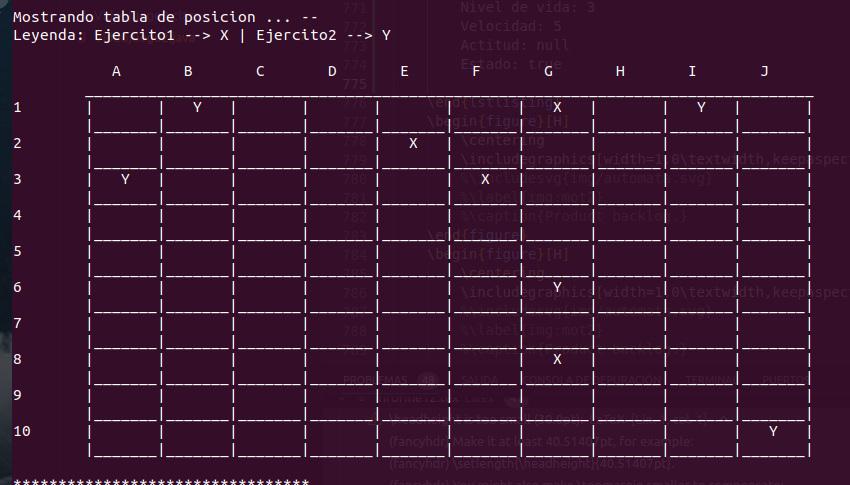
\includegraphics[width=1.0\textwidth,keepaspectratio]{img/Commit7.png}
		%\includesvg{img/automata.svg}
		%\label{img:mot2}
		%\caption{Product backlog.}
	\end{figure}
	\begin{lstlisting}[language=bash,caption={Ejecucion:}][H]
		*********************************
		Escoja una de estas opciones para el ejercito 1
		[1] Crear Soldado
		[2] Eliminar Soldado
		[3] Clonar Soldado
		[4] Modificar Soldado
		[5] Comparar Soldados
		[6] Intercambiar Soldados
		[7] Ver soldado
		[8] Ver ejercito
		[9] Sumar Niveles
		[10] Jugar
		[11] Volver
		4
		*********************************
		Escriba la fila donde esta el soldado el cual modificara:
		3
		Escriba la columna donde esta el soldado el cual modificara:
		F
		*********************************
		QUE DESEA MODIFICAR
		[1] Nivel de ataque
		[2] Nivel de defensa
		[3] Nivel de vida Actual
		2
		*********************************
		
		Nombre: Soldado3X1
		Vida: 1
		Fila: 3
		Columna: F
		Nivel de ataque: 4
		Nivel de Defensa: 5
		Nivel de vida: 1
		Velocidad: 2
		Actitud: null
		Estado: true
		*********************************
		Cual es el nivel de defensa que le pondra del 1 al 5 
		1
		*********************************
		
		Nombre: Soldado3X1
		Vida: 1
		Fila: 3
		Columna: F
		Nivel de ataque: 4
		Nivel de Defensa: 1
		Nivel de vida: 1
		Velocidad: 2
		Actitud: null
		Estado: true		
		
	\end{lstlisting}
	\begin{figure}[H]
		\centering
		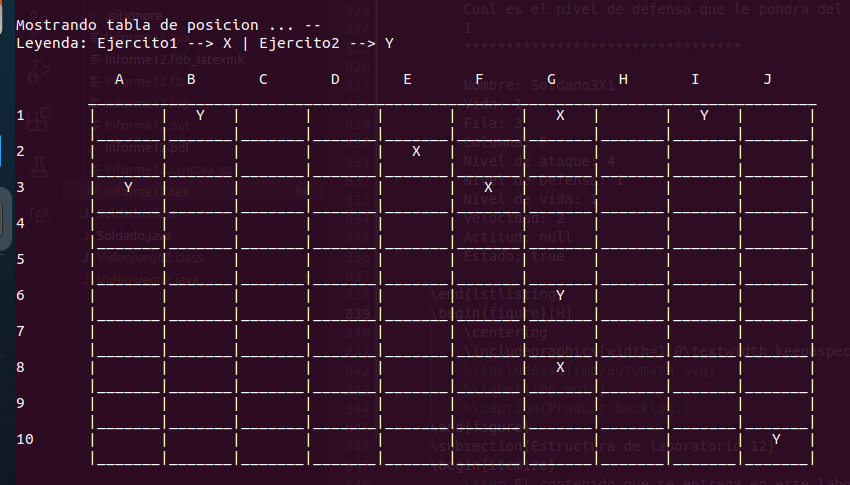
\includegraphics[width=1.0\textwidth,keepaspectratio]{img/Commit7.1.png}
		%\includesvg{img/automata.svg}
		%\label{img:mot2}
		%\caption{Product backlog.}
	\end{figure}
	\begin{lstlisting}[language=bash,caption={Ejecucion:}][H]
		*********************************
		Escoja una de estas opciones para el ejercito 1
		[1] Crear Soldado
		[2] Eliminar Soldado
		[3] Clonar Soldado
		[4] Modificar Soldado
		[5] Comparar Soldados
		[6] Intercambiar Soldados
		[7] Ver soldado
		[8] Ver ejercito
		[9] Sumar Niveles
		[10] Jugar
		[11] Volver
		4
		*********************************
		Escriba la fila donde esta el soldado el cual modificara:
		3
		Escriba la columna donde esta el soldado el cual modificara:
		F
		*********************************
		QUE DESEA MODIFICAR
		[1] Nivel de ataque
		[2] Nivel de defensa
		[3] Nivel de vida Actual
		3
		*********************************
		
		Nombre: Soldado3X1
		Vida: 1
		Fila: 3
		Columna: F
		Nivel de ataque: 4
		Nivel de Defensa: 1
		Nivel de vida: 1
		Velocidad: 2
		Actitud: null
		Estado: true
		*********************************
		Cual es el nivel de vida actual que le pondra del 1 al 5 
		5
		*********************************
		
		Nombre: Soldado3X1
		Vida: 5
		Fila: 3
		Columna: F
		Nivel de ataque: 4
		Nivel de Defensa: 1
		Nivel de vida: 1
		Velocidad: 2
		Actitud: null
		Estado: true
				
	\end{lstlisting}
	\begin{figure}[H]
		\centering
		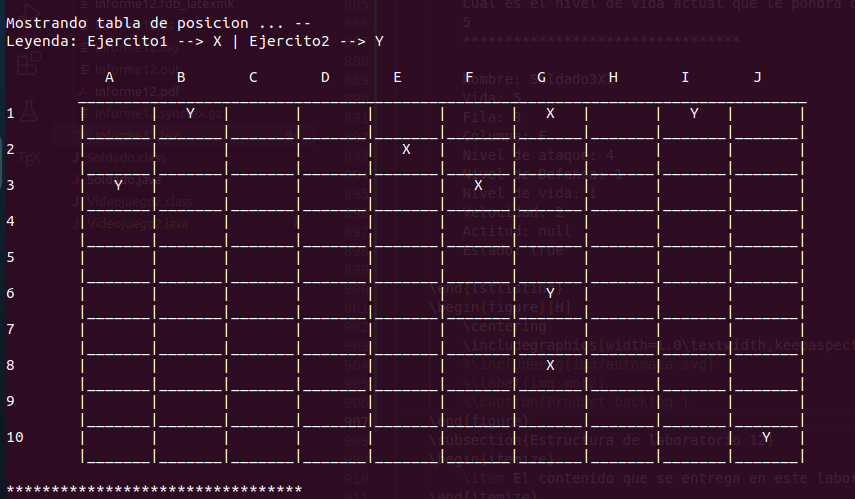
\includegraphics[width=1.0\textwidth,keepaspectratio]{img/Commit7.2.png}
		%\includesvg{img/automata.svg}
		%\label{img:mot2}
		%\caption{Product backlog.}
	\end{figure}
	\subsection{Ejercicio Videojuego2}
	\begin{itemize}	
		\item En el octavo commit agregamos la opcion 5 del menu el cual nos permite comparar soldados con algunas de sus atributos para esto solo aplicarimos condiciones y pediriamos ubicaciones
		\item El codigo , el commit y ejecucion seria el siguiente:
	\end{itemize}	
	\begin{lstlisting}[language=bash,caption={Commit}][H]
		$ git commit -m "Agregando la opcion 5 la cual nos permite comparar soldados para esto aplicamos solo condiciones para poder verificar esto"
	\end{lstlisting}	
	\begin{lstlisting}[language=java,caption={Las lineas de codigos del metodo creado:}][H]
		public static void compareSoldier(ArrayList<ArrayList<Soldado>> army){
			System.out.println("*********************************");
			Scanner sc = new Scanner(System.in);
			System.out.println("Escriba la fila donde esta el primer soldado que va comparar:");
			int row = sc.nextInt() - 1;
			System.out.println("Escriba la columna donde esta el primer soldado que va comparar:");
			String column = sc.next();
			System.out.println("EL PRIMER SOLDADO ES:");
			Soldado soldier1 = army.get(row).get((int)column.charAt(0) - 65);
			System.out.println(army.get(row).get((int)column.charAt(0) - 65).toString());
			System.out.println("\nEscriba la fila donde esta el segundo soldado que va comparar:");
			int row2 = sc.nextInt() - 1;
			System.out.println("Escriba la columna donde esta el segundo soldado que va comparar:");
			String column2 = sc.next();
			System.out.println("EL SEGUNDO SOLDADO ES:");
			Soldado soldier2 = army.get(row2).get((int)column2.charAt(0) - 65);
			System.out.println(army.get(row2).get((int)column2.charAt(0) - 65).toString());
			if(soldier1.getName().equals(soldier2.getName()) && soldier1.getAttackLevel() == soldier2.getAttackLevel() && soldier1.getDefenseLevel() == soldier2.getDefenseLevel() && soldier1.getLifeActual() == soldier2.getLifeActual() && soldier1.getLives() == soldier2.getLives()){
				System.out.println("\nLOS SOLDADOS SON IGUALES EN EL ASPECTO DE NOMBRE , NIVEL DE ATAQUE , NIVEL DE DEFENSA , NIVEL DE VIDA ACTUAL Y ESTADO");
			}else{
				System.out.println("NO SON IGUALES EN EL ASPECTO DE NOMBRE , NIVEL DE ATAQUE , NIVEL DE DEFENSA , NIVEL DE VIDA ACTUAL Y ESTADO");
			}
		}
	\end{lstlisting}
	\begin{lstlisting}[language=bash,caption={Ejecucion:}][H]
		-------------------------------------------
		--          OPCIONES DE BATALLA          --
		-------------------------------------------
		 SELECCIONE UN NUMERO PARA PODER EMPEZAR O TERMINAR
		 1 : JUEGO RAPIDO
		 2 : JUEGO PERSONALIZADO
		2
		Gestionar Ejercito 
		[1] Ejercito 1
		[2] Ejercito 2
		1
		Escoja una de estas opciones para el ejercito 1
		[1] Crear Soldado
		[2] Eliminar Soldado
		[3] Clonar Soldado
		[4] Modificar Soldado
		[5] Comparar Soldados
		[6] Intercambiar Soldados
		[7] Ver soldado
		[8] Ver ejercito
		[9] Sumar Niveles
		[10] Jugar
		[11] Volver
		5
		*********************************
		Escriba la fila donde esta el primer soldado que va comparar:
		4
		Escriba la columna donde esta el primer soldado que va comparar:
		F
		EL PRIMER SOLDADO ES:
		
		Nombre: Soldado2X1
		Vida: 2
		Fila: 4
		Columna: F
		Nivel de ataque: 2
		Nivel de Defensa: 4
		Nivel de vida: 4
		Velocidad: 3
		Actitud: null
		Estado: true
		
		Escriba la fila donde esta el segundo soldado que va comparar:
		4
		Escriba la columna donde esta el segundo soldado que va comparar:
		F
		EL SEGUNDO SOLDADO ES:
		
		Nombre: Soldado2X1
		Vida: 2
		Fila: 4
		Columna: F
		Nivel de ataque: 2
		Nivel de Defensa: 4
		Nivel de vida: 4
		Velocidad: 3
		Actitud: null
		Estado: true
		
		LOS SOLDADOS SON IGUALES EN EL ASPECTO DE NOMBRE , NIVEL DE ATAQUE , NIVEL DE DEFENSA , NIVEL DE VIDA ACTUAL Y ESTADO		
		
	\end{lstlisting}
	\begin{figure}[H]
		\centering
		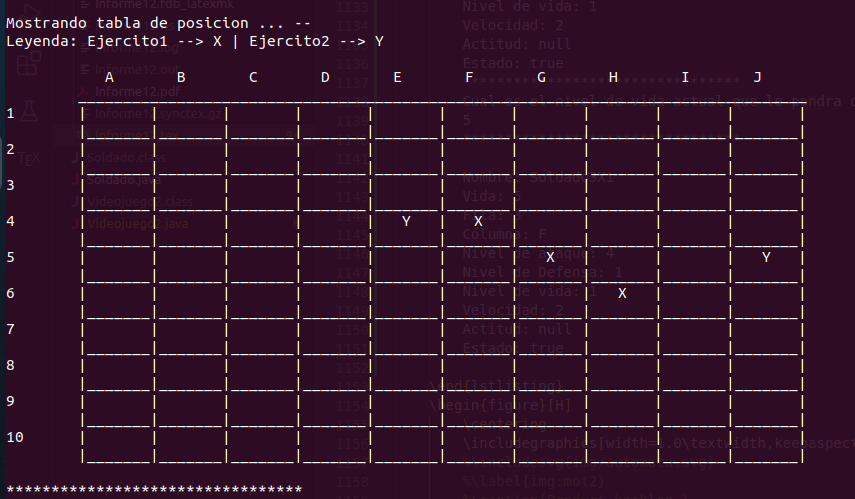
\includegraphics[width=1.0\textwidth,keepaspectratio]{img/Commit8.png}
		%\includesvg{img/automata.svg}
		%\label{img:mot2}
		%\caption{Product backlog.}
	\end{figure}
	\subsection{Ejercicio Videojuego2}
	\begin{itemize}	
		\item En el noveno commit agregamos la opcion 6 el cual intercambia posiciones de los soldados mediante el registro de sus posiciones y despues usamos un soldado el cual va a retener la referencia de uno de los soldados que va a ser eliminados para despues agregarlo en el casillero en el cual se va a intercambiar
		\item El codigo , el commit y ejecucion seria el siguiente:
	\end{itemize}	
	\begin{lstlisting}[language=bash,caption={Commit}][H]
		$ git commit -m "Agregamos la opcion 6 el cual intercambia posiciones de los soldados mediante el registro de sus posiciones y despues usamos un soldado el cual va a retener la referencia de uno de los soldados que va a ser eliminados para despues agregarlo en el casillero en el cual se va a intercambiar"
	\end{lstlisting}	
	\begin{lstlisting}[language=java,caption={Las lineas de codigos del metodo creado:}][H]
		public static void swapSoldier(ArrayList<ArrayList<Soldado>> army){
			System.out.println("*********************************");
			Scanner sc = new Scanner(System.in);
			System.out.println("Escriba la fila donde esta el primer soldado que va intercambiar de posicion:");
			int row = sc.nextInt() - 1;
			System.out.println("Escriba la columna donde esta el primer soldado que va intercambiar de posicion:");
			String column = sc.next();
			System.out.println("EL PRIMER SOLDADO ES:");
			Soldado soldier1 = army.get(row).get((int)column.charAt(0) - 65);
			System.out.println(army.get(row).get((int)column.charAt(0) - 65).toString());
			System.out.println("\nEscriba la fila donde esta el segundo soldado que va intercambiar de posicion:");
			int row2 = sc.nextInt() - 1;
			System.out.println("Escriba la columna donde esta el segundo soldado que va intercambiar de posicion:");
			String column2 = sc.next();
			System.out.println("EL SEGUNDO SOLDADO ES:");
			Soldado soldier2 = army.get(row2).get((int)column2.charAt(0) - 65);
			System.out.println(army.get(row2).get((int)column2.charAt(0) - 65).toString());
			System.out.println("*********************************");
			System.out.println("INTERCAMBIO EXITOSO");
			soldier2.setRow(row + 1);
			soldier2.setColumn(column);
			soldier1.setRow(row2 + 1);
			soldier1.setColumn(column2);
			Soldado soldiertmp = army.get(row2).get((int)column2.charAt(0) - 65);
			army.get(row2).set((int)column2.charAt(0) - 65, soldier1);
			army.get(row).set((int)column.charAt(0) - 65, soldiertmp);
			System.out.println(army.get(row).get((int)column.charAt(0) - 65).toString());
			System.out.println(army.get(row2).get((int)column2.charAt(0) - 65).toString());
		}
	\end{lstlisting}
	\begin{lstlisting}[language=bash,caption={Ejecucion:}][H]
		*********************************
		-------------------------------------------
		--          OPCIONES DE BATALLA          --
		-------------------------------------------
		 SELECCIONE UN NUMERO PARA PODER EMPEZAR O TERMINAR
		 1 : JUEGO RAPIDO
		 2 : JUEGO PERSONALIZADO
		2
		Gestionar Ejercito 
		[1] Ejercito 1
		[2] Ejercito 2
		1
		Escoja una de estas opciones para el ejercito 1
		[1] Crear Soldado
		[2] Eliminar Soldado
		[3] Clonar Soldado
		[4] Modificar Soldado
		[5] Comparar Soldados
		[6] Intercambiar Soldados
		[7] Ver soldado
		[8] Ver ejercito
		[9] Sumar Niveles
		[10] Jugar
		[11] Volver
		6
		*********************************
		Escriba la fila donde esta el primer soldado que va intercambiar de posicion:
		4
		Escriba la columna donde esta el primer soldado que va intercambiar de posicion:
		A
		EL PRIMER SOLDADO ES:
		
		Nombre: Soldado0X1
		Vida: 1
		Fila: 4
		Columna: A
		Nivel de ataque: 1
		Nivel de Defensa: 1
		Nivel de vida: 1
		Velocidad: 5
		Actitud: null
		Estado: true
		
		Escriba la fila donde esta el segundo soldado que va intercambiar de posicion:
		2
		Escriba la columna donde esta el segundo soldado que va intercambiar de posicion:
		A
		EL SEGUNDO SOLDADO ES:
		
		Nombre: Soldado5X1
		Vida: 4
		Fila: 2
		Columna: A
		Nivel de ataque: 5
		Nivel de Defensa: 4
		Nivel de vida: 4
		Velocidad: 1
		Actitud: null
		Estado: true
		INTERCAMBIO EXITOSO
		
		Nombre: Soldado5X1
		Vida: 4
		Fila: 4
		Columna: A
		Nivel de ataque: 5
		Nivel de Defensa: 4
		Nivel de vida: 4
		Velocidad: 1
		Actitud: null
		Estado: true
		
		Nombre: Soldado0X1
		Vida: 1
		Fila: 2
		Columna: A
		Nivel de ataque: 1
		Nivel de Defensa: 1
		Nivel de vida: 1
		Velocidad: 5
		Actitud: null
		Estado: true
		
		Mostrando tabla de posicion ... --
		Leyenda: Ejercito1 --> X | Ejercito2 --> Y
		
	\end{lstlisting}
	\begin{figure}[H]
		\centering
		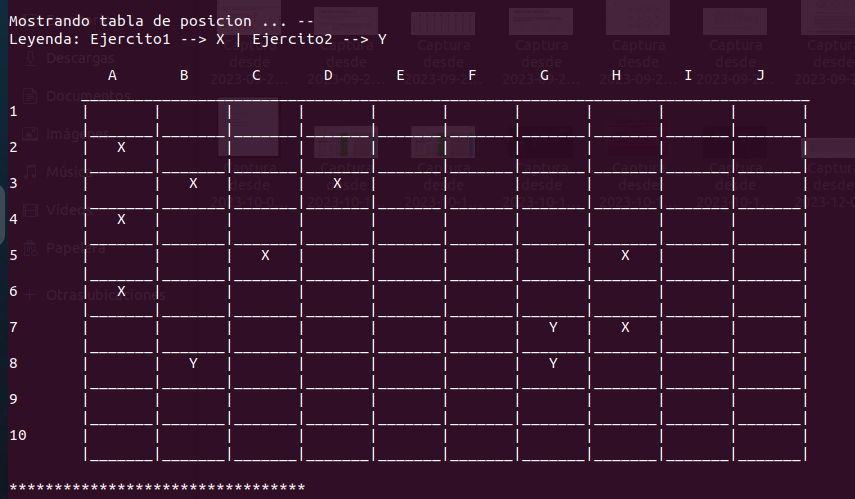
\includegraphics[width=1.0\textwidth,keepaspectratio]{img/Commit9.png}
		%\includesvg{img/automata.svg}
		%\label{img:mot2}
		%\caption{Product backlog.}
	\end{figure}
	\subsection{Ejercicio Videojuego2}
	\begin{itemize}	
		\item En el decimo commit agregamos la opcion 7 la cual nos permite buscar a un soldado para esto hacemos iteracion en cada uno de los casilleros para ver si se encontro el soldado requerido en caso de no se mostrara un mensaje
		\item El codigo , el commit y ejecucion seria el siguiente:
	\end{itemize}	
	\begin{lstlisting}[language=bash,caption={Commit}][H]
		$ git commit -m "Agregamos la opcion 7 la cual nos permite buscar a un soldado para esto hacemos iteracion en cada uno de los casilleros para ver si se encontro el soldado requerido en caso de no se mostrara un mensaje"
	\end{lstlisting}	
	\begin{lstlisting}[language=java,caption={Las lineas de codigos del metodo creado:}][H]
		public static void searchSoldier(ArrayList<ArrayList<Soldado>> army){
			Scanner sc = new Scanner(System.in);
			System.out.println("Escriba el nombre del Soldado:");
			String namesoldier = sc.next();
			int num = 0;
			for(int i = 0; i < 10; i++){  //ITERACION CREADA PARA PODER SABER QUE SI ESTE BANDO DEL EJERCITO TIENE SOLDADOS PARA PODER JUGAR SI TIENE 10 ESTA OPCION ESTA CANCELADA
				for(int j = 0; j < 10; j++){
					if(army.get(i).get(j) != null && army.get(i).get(j).getName().equals(namesoldier)){
						System.out.println("*********************************");
						System.out.println("BUSQUEDA EXITOSA \n");
						System.out.println(army.get(i).get(j));
						num++;
						break;
					}
				}
			}
			if(num == 0){
				System.out.println("*********************************");
				System.out.println("NO SE ENCONTRO AL SOLDADO \n");
			}
		}
	\end{lstlisting}
	\begin{lstlisting}[language=bash,caption={Ejecucion:}][H]
		*********************************
		-------------------------------------------
		--          OPCIONES DE BATALLA          --
		-------------------------------------------
		 SELECCIONE UN NUMERO PARA PODER EMPEZAR O TERMINAR
		 1 : JUEGO RAPIDO
		 2 : JUEGO PERSONALIZADO
		2
		Gestionar Ejercito 
		[1] Ejercito 1
		[2] Ejercito 2
		1
		Escoja una de estas opciones para el ejercito 1
		[1] Crear Soldado
		[2] Eliminar Soldado
		[3] Clonar Soldado
		[4] Modificar Soldado
		[5] Comparar Soldados
		[6] Intercambiar Soldados
		[7] Ver soldado
		[8] Ver ejercito
		[9] Sumar Niveles
		[10] Jugar
		[11] Volver
		7
		Escriba el nombre del Soldado:
		Soldado0X1
		*********************************
		BUSQUEDA EXITOSA 
		
		
		Nombre: Soldado0X1
		Vida: 1
		Fila: 6
		Columna: G
		Nivel de ataque: 1
		Nivel de Defensa: 4
		Nivel de vida: 1
		Velocidad: 1
		Actitud: null
		Estado: true		
		
	\end{lstlisting}
	\begin{figure}[H]
		\centering
		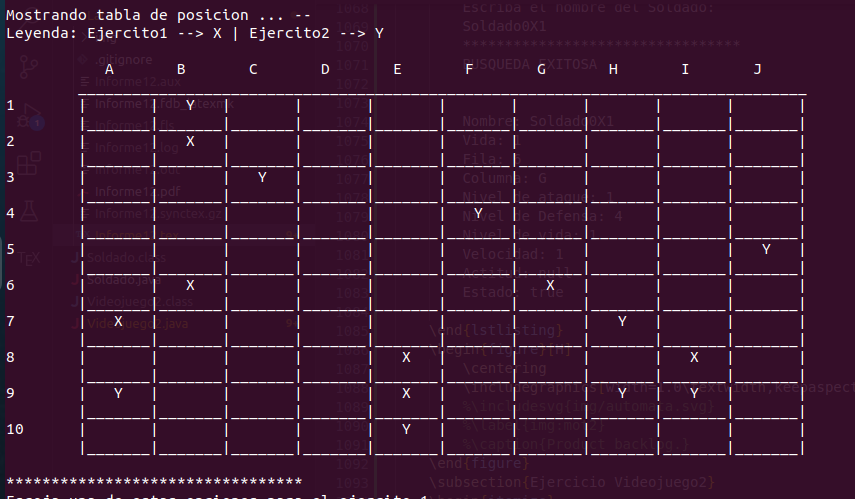
\includegraphics[width=1.0\textwidth,keepaspectratio]{img/Commit10.png}
		%\includesvg{img/automata.svg}
		%\label{img:mot2}
		%\caption{Product backlog.}
	\end{figure}
	\begin{lstlisting}[language=bash,caption={Ejecucion:}][H]
		*********************************
		Escoja una de estas opciones para el ejercito 1
		[1] Crear Soldado
		[2] Eliminar Soldado
		[3] Clonar Soldado
		[4] Modificar Soldado
		[5] Comparar Soldados
		[6] Intercambiar Soldados
		[7] Ver soldado
		[8] Ver ejercito
		[9] Sumar Niveles
		[10] Jugar
		[11] Volver
		7
		Escriba el nombre del Soldado:
		Soldado7X1
		*********************************
		NO SE ENCONTRO AL SOLDADO 
	\end{lstlisting}
	\begin{figure}[H]
		\centering
		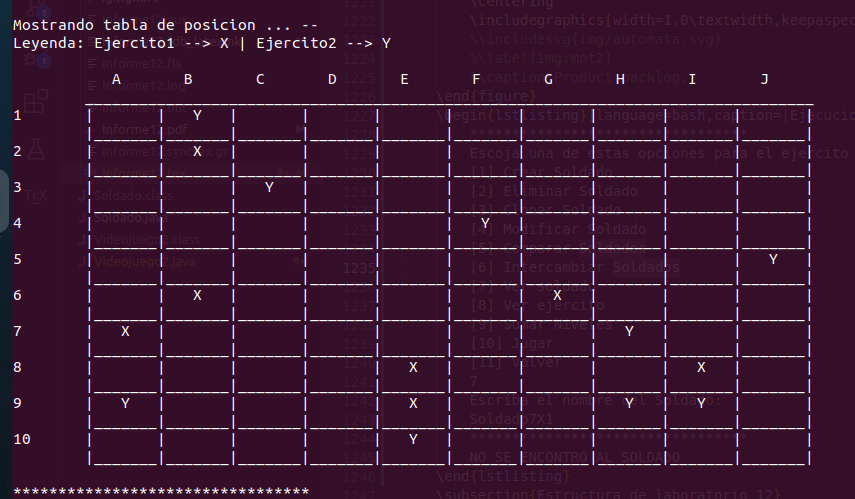
\includegraphics[width=1.0\textwidth,keepaspectratio]{img/Commit10.1.png}
		%\includesvg{img/automata.svg}
		%\label{img:mot2}
		%\caption{Product backlog.}
	\end{figure}
	\subsection{Estructura de laboratorio 12}
	\begin{itemize}	
		\item El contenido que se entrega en este laboratorio12 es el siguiente:
	\end{itemize}
	\begin{lstlisting}[style=ascii-tree]
	/Lab12	

	\end{lstlisting}    
	\section{\textcolor{red}{Rúbricas}}
	
	\subsection{\textcolor{red}{Entregable Informe}}
	\begin{table}[H]
		\caption{Tipo de Informe}
		\setlength{\tabcolsep}{0.5em} % for the horizontal padding
		{\renewcommand{\arraystretch}{1.5}% for the vertical padding
		\begin{tabular}{|p{3cm}|p{12cm}|}
			\hline
			\multicolumn{2}{|c|}{\textbf{\textcolor{red}{Informe}}}  \\
			\hline 
			\textbf{\textcolor{red}{Latex}} & \textcolor{blue}{El informe está en formato PDF desde Latex,  con un formato limpio (buena presentación) y facil de leer.}   \\ 
			\hline 
			
			
		\end{tabular}
	}
	\end{table}
	
	\clearpage
	
	\subsection{\textcolor{red}{Rúbrica para el contenido del Informe y demostración}}
	\begin{itemize}			
		\item El alumno debe marcar o dejar en blanco en celdas de la columna \textbf{Checklist} si cumplio con el ítem correspondiente.
		\item Si un alumno supera la fecha de entrega,  su calificación será sobre la nota mínima aprobada, siempre y cuando cumpla con todos lo items.
		\item El alumno debe autocalificarse en la columna \textbf{Estudiante} de acuerdo a la siguiente tabla:
	
		\begin{table}[ht]
			\caption{Niveles de desempeño}
			\begin{center}
			\begin{tabular}{ccccc}
    			\hline
    			 & \multicolumn{4}{c}{Nivel}\\
    			\cline{1-5}
    			\textbf{Puntos} & Insatisfactorio 25\%& En Proceso 50\% & Satisfactorio 75\% & Sobresaliente 100\%\\
    			\textbf{2.0}&0.5&1.0&1.5&2.0\\
    			\textbf{4.0}&1.0&2.0&3.0&4.0\\
    		\hline
			\end{tabular}
		\end{center}
	\end{table}	
	
	\end{itemize}
	
	\begin{table}[H]
		\caption{Rúbrica para contenido del Informe y demostración}
		\setlength{\tabcolsep}{0.5em} % for the horizontal padding
		{\renewcommand{\arraystretch}{1.5}% for the vertical padding
		%\begin{center}
		\begin{tabular}{|p{2.7cm}|p{7cm}|x{1.3cm}|p{1.2cm}|p{1.5cm}|p{1.1cm}|}
			\hline
    		\multicolumn{2}{|c|}{Contenido y demostración} & Puntos & Checklist & Estudiante & Profesor\\
			\hline
			\textbf{1. GitHub} & Hay enlace URL activo del directorio para el  laboratorio hacia su repositorio GitHub con código fuente terminado y fácil de revisar. &2 &X &2 & \\ 
			\hline
			\textbf{2. Commits} &  Hay capturas de pantalla de los commits más importantes con sus explicaciones detalladas. (El profesor puede preguntar para refrendar calificación). &4 &X &4 & \\ 
			\hline 
			\textbf{3. Código fuente} &  Hay porciones de código fuente importantes con numeración y explicaciones detalladas de sus funciones. &2 &X &2 & \\ 
			\hline 
			\textbf{4. Ejecución} & Se incluyen ejecuciones/pruebas del código fuente  explicadas gradualmente. &2 &X &2 & \\ 
			\hline			
			\textbf{5. Pregunta} & Se responde con completitud a la pregunta formulada en la tarea.  (El profesor puede preguntar para refrendar calificación).  &2 &X &2 & \\ 
			\hline	
			\textbf{6. Fechas} & Las fechas de modificación del código fuente estan dentro de los plazos de fecha de entrega establecidos. &2 &X &2 & \\ 
			\hline 
			\textbf{7. Ortografía} & El documento no muestra errores ortográficos. &2 &X &2 & \\ 
			\hline 
			\textbf{8. Madurez} & El Informe muestra de manera general una evolución de la madurez del código fuente,  explicaciones puntuales pero precisas y un acabado impecable.   (El profesor puede preguntar para refrendar calificación).  &4 &X &2 & \\ 
			\hline
			\multicolumn{2}{|c|}{\textbf{Total}} &20 & &18 & \\ 
			\hline
		\end{tabular}
		%\end{center}
		%\label{tab:multicol}
		}
	\end{table}
	
\clearpage

\section{Referencias}
\begin{itemize}			
	\item \url{https://drive.google.com/drive/u/1/folders/19TzLFO-T77qG7bOWmg5OH7FXAMD2CrJL}
\end{itemize}	
	
%\clearpage
%\bibliographystyle{apalike}
%\bibliographystyle{IEEEtranN}
%\bibliography{bibliography}
			
\end{document}